\documentclass[]{article}
\usepackage{lmodern}
\usepackage{amssymb,amsmath}
\usepackage{ifxetex,ifluatex}
\usepackage{fixltx2e} % provides \textsubscript
\ifnum 0\ifxetex 1\fi\ifluatex 1\fi=0 % if pdftex
  \usepackage[T1]{fontenc}
  \usepackage[utf8]{inputenc}
\else % if luatex or xelatex
  \ifxetex
    \usepackage{mathspec}
  \else
    \usepackage{fontspec}
  \fi
  \defaultfontfeatures{Ligatures=TeX,Scale=MatchLowercase}
\fi
% use upquote if available, for straight quotes in verbatim environments
\IfFileExists{upquote.sty}{\usepackage{upquote}}{}
% use microtype if available
\IfFileExists{microtype.sty}{%
\usepackage{microtype}
\UseMicrotypeSet[protrusion]{basicmath} % disable protrusion for tt fonts
}{}
\usepackage[margin=1in]{geometry}
\usepackage{hyperref}
\hypersetup{unicode=true,
            pdftitle={Identificando outliers},
            pdfauthor={Carlos Eduardo Barbosa},
            pdfborder={0 0 0},
            breaklinks=true}
\urlstyle{same}  % don't use monospace font for urls
\usepackage{color}
\usepackage{fancyvrb}
\newcommand{\VerbBar}{|}
\newcommand{\VERB}{\Verb[commandchars=\\\{\}]}
\DefineVerbatimEnvironment{Highlighting}{Verbatim}{commandchars=\\\{\}}
% Add ',fontsize=\small' for more characters per line
\usepackage{framed}
\definecolor{shadecolor}{RGB}{248,248,248}
\newenvironment{Shaded}{\begin{snugshade}}{\end{snugshade}}
\newcommand{\AlertTok}[1]{\textcolor[rgb]{0.94,0.16,0.16}{#1}}
\newcommand{\AnnotationTok}[1]{\textcolor[rgb]{0.56,0.35,0.01}{\textbf{\textit{#1}}}}
\newcommand{\AttributeTok}[1]{\textcolor[rgb]{0.77,0.63,0.00}{#1}}
\newcommand{\BaseNTok}[1]{\textcolor[rgb]{0.00,0.00,0.81}{#1}}
\newcommand{\BuiltInTok}[1]{#1}
\newcommand{\CharTok}[1]{\textcolor[rgb]{0.31,0.60,0.02}{#1}}
\newcommand{\CommentTok}[1]{\textcolor[rgb]{0.56,0.35,0.01}{\textit{#1}}}
\newcommand{\CommentVarTok}[1]{\textcolor[rgb]{0.56,0.35,0.01}{\textbf{\textit{#1}}}}
\newcommand{\ConstantTok}[1]{\textcolor[rgb]{0.00,0.00,0.00}{#1}}
\newcommand{\ControlFlowTok}[1]{\textcolor[rgb]{0.13,0.29,0.53}{\textbf{#1}}}
\newcommand{\DataTypeTok}[1]{\textcolor[rgb]{0.13,0.29,0.53}{#1}}
\newcommand{\DecValTok}[1]{\textcolor[rgb]{0.00,0.00,0.81}{#1}}
\newcommand{\DocumentationTok}[1]{\textcolor[rgb]{0.56,0.35,0.01}{\textbf{\textit{#1}}}}
\newcommand{\ErrorTok}[1]{\textcolor[rgb]{0.64,0.00,0.00}{\textbf{#1}}}
\newcommand{\ExtensionTok}[1]{#1}
\newcommand{\FloatTok}[1]{\textcolor[rgb]{0.00,0.00,0.81}{#1}}
\newcommand{\FunctionTok}[1]{\textcolor[rgb]{0.00,0.00,0.00}{#1}}
\newcommand{\ImportTok}[1]{#1}
\newcommand{\InformationTok}[1]{\textcolor[rgb]{0.56,0.35,0.01}{\textbf{\textit{#1}}}}
\newcommand{\KeywordTok}[1]{\textcolor[rgb]{0.13,0.29,0.53}{\textbf{#1}}}
\newcommand{\NormalTok}[1]{#1}
\newcommand{\OperatorTok}[1]{\textcolor[rgb]{0.81,0.36,0.00}{\textbf{#1}}}
\newcommand{\OtherTok}[1]{\textcolor[rgb]{0.56,0.35,0.01}{#1}}
\newcommand{\PreprocessorTok}[1]{\textcolor[rgb]{0.56,0.35,0.01}{\textit{#1}}}
\newcommand{\RegionMarkerTok}[1]{#1}
\newcommand{\SpecialCharTok}[1]{\textcolor[rgb]{0.00,0.00,0.00}{#1}}
\newcommand{\SpecialStringTok}[1]{\textcolor[rgb]{0.31,0.60,0.02}{#1}}
\newcommand{\StringTok}[1]{\textcolor[rgb]{0.31,0.60,0.02}{#1}}
\newcommand{\VariableTok}[1]{\textcolor[rgb]{0.00,0.00,0.00}{#1}}
\newcommand{\VerbatimStringTok}[1]{\textcolor[rgb]{0.31,0.60,0.02}{#1}}
\newcommand{\WarningTok}[1]{\textcolor[rgb]{0.56,0.35,0.01}{\textbf{\textit{#1}}}}
\usepackage{graphicx,grffile}
\makeatletter
\def\maxwidth{\ifdim\Gin@nat@width>\linewidth\linewidth\else\Gin@nat@width\fi}
\def\maxheight{\ifdim\Gin@nat@height>\textheight\textheight\else\Gin@nat@height\fi}
\makeatother
% Scale images if necessary, so that they will not overflow the page
% margins by default, and it is still possible to overwrite the defaults
% using explicit options in \includegraphics[width, height, ...]{}
\setkeys{Gin}{width=\maxwidth,height=\maxheight,keepaspectratio}
\IfFileExists{parskip.sty}{%
\usepackage{parskip}
}{% else
\setlength{\parindent}{0pt}
\setlength{\parskip}{6pt plus 2pt minus 1pt}
}
\setlength{\emergencystretch}{3em}  % prevent overfull lines
\providecommand{\tightlist}{%
  \setlength{\itemsep}{0pt}\setlength{\parskip}{0pt}}
\setcounter{secnumdepth}{0}
% Redefines (sub)paragraphs to behave more like sections
\ifx\paragraph\undefined\else
\let\oldparagraph\paragraph
\renewcommand{\paragraph}[1]{\oldparagraph{#1}\mbox{}}
\fi
\ifx\subparagraph\undefined\else
\let\oldsubparagraph\subparagraph
\renewcommand{\subparagraph}[1]{\oldsubparagraph{#1}\mbox{}}
\fi

%%% Use protect on footnotes to avoid problems with footnotes in titles
\let\rmarkdownfootnote\footnote%
\def\footnote{\protect\rmarkdownfootnote}

%%% Change title format to be more compact
\usepackage{titling}

% Create subtitle command for use in maketitle
\newcommand{\subtitle}[1]{
  \posttitle{
    \begin{center}\large#1\end{center}
    }
}

\setlength{\droptitle}{-2em}

  \title{Identificando outliers}
    \pretitle{\vspace{\droptitle}\centering\huge}
  \posttitle{\par}
    \author{Carlos Eduardo Barbosa}
    \preauthor{\centering\large\emph}
  \postauthor{\par}
      \predate{\centering\large\emph}
  \postdate{\par}
    \date{08/12/2019}


\begin{document}
\maketitle

Em estatística, o \textbf{outlier} (também conhecidos como \textbf{valor
aberrante} ou \textbf{valor atípico}) é uma observação que apresenta uma
grande diferença dos demais valores ou até mesmo inconsistente.

A existência de \emph{outliers} implica em uma interpretação errada dos
resultados estatísticos.

Existem vários métodos de identificação de \emph{outliers}, nesse artigo
vamos utilizar o gráfico de \texttt{boxplot.stats} e \texttt{hist}.

Para uma melhor apresentação e comparação, vamos criar um método chamado
\texttt{outlierInfo} que plota os gráficos com e sem os outliers, com
isso, temos uma visão mais nítida comparando os dados.

\begin{Shaded}
\begin{Highlighting}[]
\CommentTok{#outlierInfo: fornece uma analise sobre possiveis outliers em um dado}
\NormalTok{outlierInfo <-}\StringTok{ }\ControlFlowTok{function}\NormalTok{(dt, var, }\DataTypeTok{labelName =} \StringTok{""}\NormalTok{, }\DataTypeTok{showMessage =} \OtherTok{FALSE}\NormalTok{, }\DataTypeTok{removeOutlier =} \OtherTok{FALSE}\NormalTok{) \{}
\NormalTok{    varName <-}\StringTok{ }\KeywordTok{eval}\NormalTok{(}\KeywordTok{substitute}\NormalTok{(var), }\KeywordTok{eval}\NormalTok{(dt))}

\NormalTok{    tot <-}\StringTok{ }\KeywordTok{sum}\NormalTok{(}\OperatorTok{!}\KeywordTok{is.na}\NormalTok{(varName)) }\CommentTok{#Total de itens nao null}
\NormalTok{    na1 <-}\StringTok{ }\KeywordTok{sum}\NormalTok{(}\KeywordTok{is.na}\NormalTok{(varName)) }\CommentTok{#Total de itens null}
\NormalTok{    m1 <-}\StringTok{ }\KeywordTok{mean}\NormalTok{(varName, }\DataTypeTok{na.rm =}\NormalTok{ T) }\CommentTok{#Media dos itens}

    \CommentTok{#Criando grafico com os outliers}
    \KeywordTok{par}\NormalTok{(}\DataTypeTok{mfrow =} \KeywordTok{c}\NormalTok{(}\DecValTok{2}\NormalTok{, }\DecValTok{2}\NormalTok{), }\DataTypeTok{oma =} \KeywordTok{c}\NormalTok{(}\DecValTok{0}\NormalTok{, }\DecValTok{0}\NormalTok{, }\DecValTok{3}\NormalTok{, }\DecValTok{0}\NormalTok{))}
    \KeywordTok{boxplot}\NormalTok{(varName, }\DataTypeTok{main =} \StringTok{"Boxplot com outliers"}\NormalTok{)}
    \KeywordTok{hist}\NormalTok{(varName, }\DataTypeTok{main =} \StringTok{"Histograma com outliers"}\NormalTok{, }\DataTypeTok{xlab =} \OtherTok{NA}\NormalTok{, }\DataTypeTok{ylab =} \OtherTok{NA}\NormalTok{)}
\NormalTok{    outlier <-}\StringTok{ }\KeywordTok{boxplot.stats}\NormalTok{(varName)}\OperatorTok{$}\NormalTok{out}

    \CommentTok{#Criando grafico sem os outliers}
\NormalTok{    varName <-}\StringTok{ }\KeywordTok{ifelse}\NormalTok{(varName }\OperatorTok\StringTok{ }\NormalTok{outlier, }\OtherTok{NA}\NormalTok{, varName)}
    \KeywordTok{boxplot}\NormalTok{(varName, }\DataTypeTok{main =} \StringTok{"Boxplot sem outliers"}\NormalTok{)}
    \KeywordTok{hist}\NormalTok{(varName, }\DataTypeTok{main =} \StringTok{"Histograma sem outliers"}\NormalTok{, }\DataTypeTok{xlab =} \OtherTok{NA}\NormalTok{, }\DataTypeTok{ylab =} \OtherTok{NA}\NormalTok{)}
    \KeywordTok{title}\NormalTok{(}\KeywordTok{paste}\NormalTok{(labelName, }\StringTok{"Outlier Check"}\NormalTok{), }\DataTypeTok{outer =} \OtherTok{TRUE}\NormalTok{)}
\NormalTok{    na2 <-}\StringTok{ }\KeywordTok{sum}\NormalTok{(}\KeywordTok{is.na}\NormalTok{(varName))}

    \CommentTok{#Calculando dados com e sem outliers}
\NormalTok{    outliersCount =}\StringTok{ }\NormalTok{na2 }\OperatorTok{-}\StringTok{ }\NormalTok{na1}
\NormalTok{    outliersPercent =}\StringTok{ }\NormalTok{((na2 }\OperatorTok{-}\StringTok{ }\NormalTok{na1) }\OperatorTok{/}\StringTok{ }\NormalTok{tot }\OperatorTok{*}\StringTok{ }\DecValTok{100}\NormalTok{)}
\NormalTok{    meanoutliers <-}\StringTok{ }\KeywordTok{mean}\NormalTok{(outlier)}
\NormalTok{    meanWithOutliers =}\StringTok{ }\NormalTok{m1}
\NormalTok{    meanWithoutOutliers =}\StringTok{ }\KeywordTok{mean}\NormalTok{(varName, }\DataTypeTok{na.rm =}\NormalTok{ T)}

    \CommentTok{#Remove os outliers conforme o parametro}
    \ControlFlowTok{if}\NormalTok{ (removeOutlier) \{}
\NormalTok{        dt[}\KeywordTok{as.character}\NormalTok{(}\KeywordTok{substitute}\NormalTok{(var))] <-}\StringTok{ }\KeywordTok{invisible}\NormalTok{(var_name)}
        \KeywordTok{assign}\NormalTok{(}\KeywordTok{as.character}\NormalTok{(}\KeywordTok{as.list}\NormalTok{(}\KeywordTok{match.call}\NormalTok{())}\OperatorTok{$}\NormalTok{dt), dt, }\DataTypeTok{envir =}\NormalTok{ .GlobalEnv)}
\NormalTok{    \}}

    \CommentTok{#Apresenta informações sobre os dados conforme o paramtro}
    \ControlFlowTok{if}\NormalTok{ (showMessage) \{}
        \KeywordTok{message}\NormalTok{(labelName, }\StringTok{" observations:"}\NormalTok{)}
        \KeywordTok{message}\NormalTok{(}\StringTok{"Outliers identified: "}\NormalTok{, outliersCount, }\StringTok{" from "}\NormalTok{, tot, }\StringTok{" observations"}\NormalTok{)}
        \KeywordTok{message}\NormalTok{(}\StringTok{"Proportion (%) of outliers: "}\NormalTok{, outliersPercent)}
        \KeywordTok{message}\NormalTok{(}\StringTok{"Mean of the outliers: "}\NormalTok{, meanoutliers)}
        \KeywordTok{message}\NormalTok{(}\StringTok{"Mean with outliers: "}\NormalTok{, meanWithOutliers)}
        \KeywordTok{message}\NormalTok{(}\StringTok{"Mean without outliers: "}\NormalTok{, meanWithoutOutliers)}
\NormalTok{    \}}

    \CommentTok{#Crio variavel de retorno}
\NormalTok{    results <-}\StringTok{ }\KeywordTok{list}\NormalTok{()}

    \CommentTok{#Preencho os dados da variavel de retorno}
\NormalTok{    results}\OperatorTok{$}\NormalTok{withoutOutliers <-}\StringTok{ }\NormalTok{varName[}\OperatorTok{!}\KeywordTok{is.na}\NormalTok{(varName)]}
\NormalTok{    results}\OperatorTok{$}\NormalTok{withOutliers <-}\StringTok{ }\NormalTok{var}
\NormalTok{    results}\OperatorTok{$}\NormalTok{outliers <-}\StringTok{ }\NormalTok{outlier}
\NormalTok{    results}\OperatorTok{$}\NormalTok{outliersCount <-}\StringTok{ }\NormalTok{outliersCount}
\NormalTok{    results}\OperatorTok{$}\NormalTok{outliersPercent <-}\StringTok{ }\NormalTok{outliersPercent}
\NormalTok{    results}\OperatorTok{$}\NormalTok{meanoutliers <-}\StringTok{ }\NormalTok{meanoutliers}
\NormalTok{    results}\OperatorTok{$}\NormalTok{meanWithOutliers <-}\StringTok{ }\NormalTok{meanWithOutliers}
\NormalTok{    results}\OperatorTok{$}\NormalTok{meanWithoutOutliers <-}\StringTok{ }\NormalTok{meanWithoutOutliers}

    \CommentTok{#Retorno a variavel}
    \KeywordTok{return}\NormalTok{(}\KeywordTok{invisible}\NormalTok{(results));}
\NormalTok{\}}
\end{Highlighting}
\end{Shaded}

Após criado o método, vamos criar o dataframe com os dados do
\emph{outliers} na variável \texttt{dataOutliers}.

\begin{Shaded}
\begin{Highlighting}[]
\NormalTok{dataOutliers <-}\StringTok{ }\KeywordTok{data.frame}\NormalTok{(}\DataTypeTok{speed =} \KeywordTok{c}\NormalTok{(}\DecValTok{18}\NormalTok{, }\DecValTok{19}\NormalTok{, }\DecValTok{19}\NormalTok{, }\DecValTok{20}\NormalTok{, }\DecValTok{20}\NormalTok{, }\DecValTok{20}\NormalTok{, }\DecValTok{23}\NormalTok{, }\DecValTok{22}\NormalTok{, }\DecValTok{25}\NormalTok{, }\DecValTok{25}\NormalTok{), }\DataTypeTok{dist =} \KeywordTok{c}\NormalTok{(}\DecValTok{183}\NormalTok{, }\DecValTok{190}\NormalTok{, }\DecValTok{186}\NormalTok{, }\DecValTok{210}\NormalTok{, }\DecValTok{220}\NormalTok{, }\DecValTok{218}\NormalTok{, }\DecValTok{220}\NormalTok{, }\DecValTok{200}\NormalTok{, }\DecValTok{1200}\NormalTok{, }\DecValTok{1250}\NormalTok{))}
\end{Highlighting}
\end{Shaded}

O dataframe possui 2 colunas, \emph{speed} e \emph{dist}, onde na coluna
\emph{speed} passamos os valores
\texttt{{[}18,\ 19,\ 19,\ 20,\ 20,\ 20,\ 23,\ 22,\ 25,\ 25{]}} e na
coluna \emph{dist} passamos os valores
\texttt{{[}183,190,\ 186,\ 210,\ 220,\ 218,\ 220,\ 200,\ 1200,\ 1250{]}}.

O dataframe possui 2 colunas, \emph{speed} e \emph{dist}, onde na coluna
\emph{speed} passamos os valores
\texttt{{[}18,\ 19,\ 19,\ 20,\ 20,\ 20,\ 23,\ 22,\ 25,\ 25{]}} e na
coluna \emph{dist} passamos os valores
\texttt{{[}183,190,\ 186,\ 210,\ 220,\ 218,\ 220,\ 200,\ 1200,\ 1250{]}}.

Após criado o dataFrame, vamos chamar o método outlierInfo e passar os
parâmetros:

\begin{itemize}
\tightlist
\item
  dataOutliers (dataFrame para analise)
\item
  dataOutliers.dist (coluna do dataFrame para analise)
\item
  Carros -- Distancia (título do gráfico)
\item
  FALSE (informar os dados no console)
\end{itemize}

\begin{Shaded}
\begin{Highlighting}[]
\NormalTok{result <-}\StringTok{ }\KeywordTok{outlierInfo}\NormalTok{(dataOutliers, dataOutliers}\OperatorTok{$}\NormalTok{dist, }\StringTok{"Carros - Distancia"}\NormalTok{, }\OtherTok{FALSE}\NormalTok{)}
\end{Highlighting}
\end{Shaded}

\includegraphics{Portifolio_Outlier_files/figure-latex/unnamed-chunk-3-1.pdf}

\hypertarget{analisando-os-dados}{%
\subsection{Analisando os dados}\label{analisando-os-dados}}

Se olharmos os dados originais, que são representados pelos gráficos
\texttt{Boxplot\ com\ outliers} e \texttt{Histograma\ com\ outliers},
temos no gráfico \texttt{Boxplot\ com\ outliers} 2 pontos na parte
superior enquanto que no \texttt{Histograma\ com\ outliers} temos um
gráfico irregular.

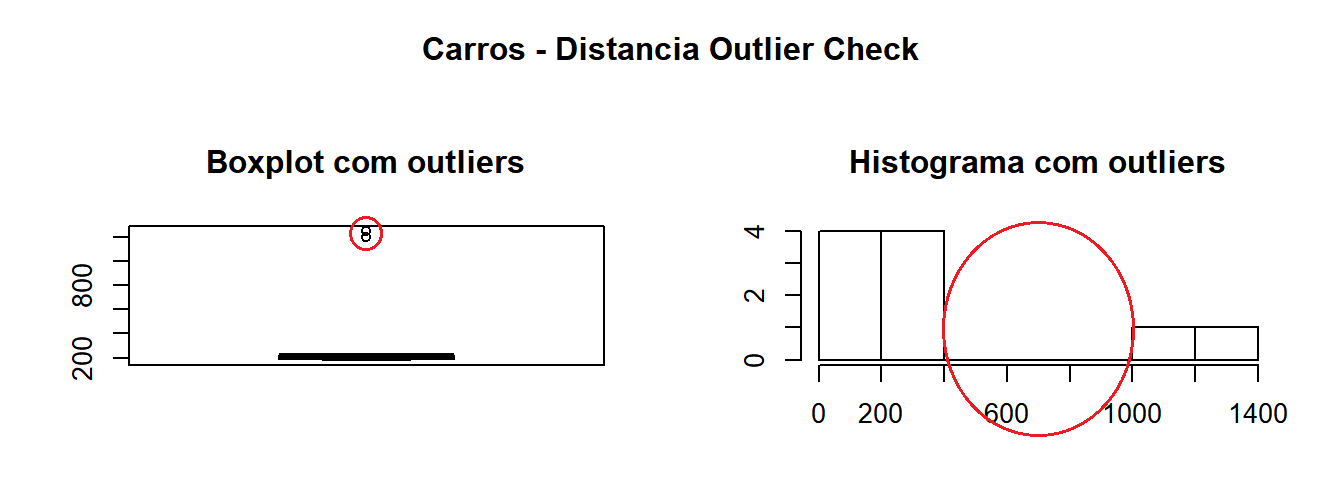
\includegraphics{Portifolio_Outlier_outlierInfo_result_com_outlier.png}

Nos dados tratados, temos os gráficos \texttt{Boxplot\ sem\ outliers} e
\texttt{Histograma\ sem\ outliers}. No gráfico
\texttt{Boxplot\ sem\ outliers} vemos que os 2 pontos na parte superior
sumiram enquanto que no \texttt{Histograma\ com\ outliers} temos uma
distribuição regular.

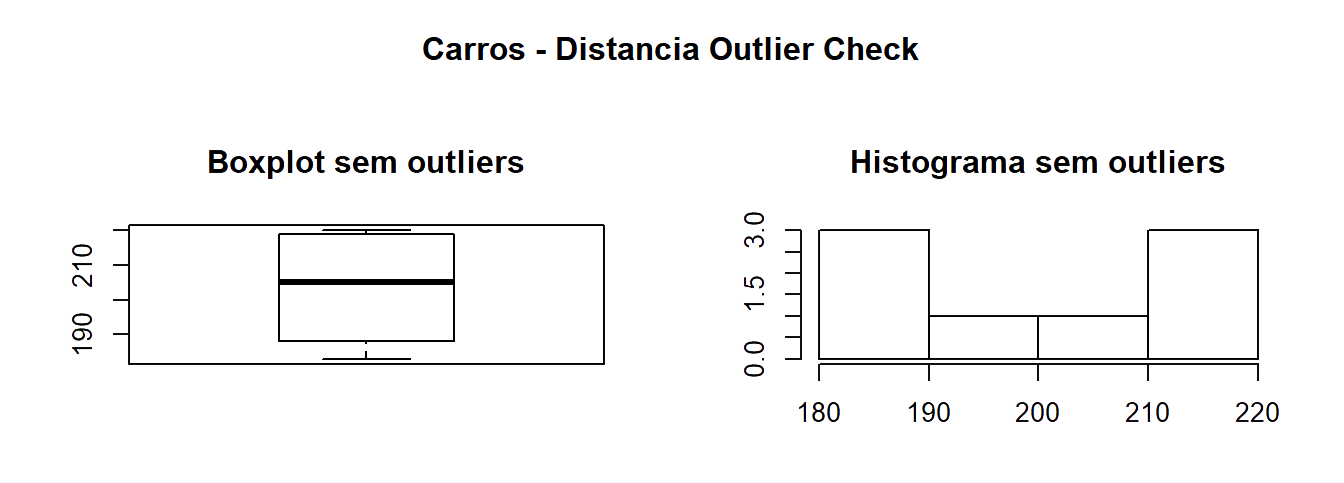
\includegraphics{Portifolio_Outlier_outlierInfo_result_sem_outlier.png}

\hypertarget{conclusao}{%
\subsection{Conclusão}\label{conclusao}}

Utilizando os gráficos \texttt{boxplot.stats} e \texttt{hist} temos uma
visão rápida e direta dos dados e com a método \texttt{outlierInfo} que
criamos, conseguimos comparar visualmente como seriam os dados com e sem
outlers.


\end{document}
